\documentclass[twoside]{book}

% Packages required by doxygen
\usepackage{fixltx2e}
\usepackage{calc}
\usepackage{doxygen}
\usepackage[export]{adjustbox} % also loads graphicx
\usepackage{graphicx}
\usepackage[utf8]{inputenc}
\usepackage{makeidx}
\usepackage{multicol}
\usepackage{multirow}
\PassOptionsToPackage{warn}{textcomp}
\usepackage{textcomp}
\usepackage[nointegrals]{wasysym}
\usepackage[table]{xcolor}

% Font selection
\usepackage[T1]{fontenc}
\usepackage[scaled=.90]{helvet}
\usepackage{courier}
\usepackage{amssymb}
\usepackage{sectsty}
\renewcommand{\familydefault}{\sfdefault}
\allsectionsfont{%
  \fontseries{bc}\selectfont%
  \color{darkgray}%
}
\renewcommand{\DoxyLabelFont}{%
  \fontseries{bc}\selectfont%
  \color{darkgray}%
}
\newcommand{\+}{\discretionary{\mbox{\scriptsize$\hookleftarrow$}}{}{}}

% Page & text layout
\usepackage{geometry}
\geometry{%
  a4paper,%
  top=2.5cm,%
  bottom=2.5cm,%
  left=2.5cm,%
  right=2.5cm%
}
\tolerance=750
\hfuzz=15pt
\hbadness=750
\setlength{\emergencystretch}{15pt}
\setlength{\parindent}{0cm}
\setlength{\parskip}{3ex plus 2ex minus 2ex}
\makeatletter
\renewcommand{\paragraph}{%
  \@startsection{paragraph}{4}{0ex}{-1.0ex}{1.0ex}{%
    \normalfont\normalsize\bfseries\SS@parafont%
  }%
}
\renewcommand{\subparagraph}{%
  \@startsection{subparagraph}{5}{0ex}{-1.0ex}{1.0ex}{%
    \normalfont\normalsize\bfseries\SS@subparafont%
  }%
}
\makeatother

% Headers & footers
\usepackage{fancyhdr}
\pagestyle{fancyplain}
\fancyhead[LE]{\fancyplain{}{\bfseries\thepage}}
\fancyhead[CE]{\fancyplain{}{}}
\fancyhead[RE]{\fancyplain{}{\bfseries\leftmark}}
\fancyhead[LO]{\fancyplain{}{\bfseries\rightmark}}
\fancyhead[CO]{\fancyplain{}{}}
\fancyhead[RO]{\fancyplain{}{\bfseries\thepage}}
\fancyfoot[LE]{\fancyplain{}{}}
\fancyfoot[CE]{\fancyplain{}{}}
\fancyfoot[RE]{\fancyplain{}{\bfseries\scriptsize Generated by Doxygen }}
\fancyfoot[LO]{\fancyplain{}{\bfseries\scriptsize Generated by Doxygen }}
\fancyfoot[CO]{\fancyplain{}{}}
\fancyfoot[RO]{\fancyplain{}{}}
\renewcommand{\footrulewidth}{0.4pt}
\renewcommand{\chaptermark}[1]{%
  \markboth{#1}{}%
}
\renewcommand{\sectionmark}[1]{%
  \markright{\thesection\ #1}%
}

% Indices & bibliography
\usepackage{natbib}
\usepackage[titles]{tocloft}
\setcounter{tocdepth}{3}
\setcounter{secnumdepth}{5}
\makeindex

% Hyperlinks (required, but should be loaded last)
\usepackage{ifpdf}
\ifpdf
  \usepackage[pdftex,pagebackref=true]{hyperref}
\else
  \usepackage[ps2pdf,pagebackref=true]{hyperref}
\fi
\hypersetup{%
  colorlinks=true,%
  linkcolor=blue,%
  citecolor=blue,%
  unicode%
}

% Custom commands
\newcommand{\clearemptydoublepage}{%
  \newpage{\pagestyle{empty}\cleardoublepage}%
}

\usepackage{caption}
\captionsetup{labelsep=space,justification=centering,font={bf},singlelinecheck=off,skip=4pt,position=top}

%===== C O N T E N T S =====

\begin{document}

% Titlepage & ToC
\hypersetup{pageanchor=false,
             bookmarksnumbered=true,
             pdfencoding=unicode
            }
\pagenumbering{roman}
\begin{titlepage}
\vspace*{7cm}
\begin{center}%
{\Large My Project }\\
\vspace*{1cm}
{\large Generated by Doxygen 1.8.11}\\
\end{center}
\end{titlepage}
\clearemptydoublepage
\tableofcontents
\clearemptydoublepage
\pagenumbering{arabic}
\hypersetup{pageanchor=true}

%--- Begin generated contents ---
\chapter{Class Index}
\section{Class List}
Here are the classes, structs, unions and interfaces with brief descriptions\+:\begin{DoxyCompactList}
\item\contentsline{section}{\hyperlink{class_fan}{Fan} }{\pageref{class_fan}}{}
\item\contentsline{section}{\hyperlink{class_l_x4__4}{L\+X4\+\_\+4} }{\pageref{class_l_x4__4}}{}
\end{DoxyCompactList}

\chapter{File Index}
\section{File List}
Here is a list of all files with brief descriptions\+:\begin{DoxyCompactList}
\item\contentsline{section}{source\+\_\+directory/fan/\hyperlink{_fan_8java}{Fan.\+java} }{\pageref{_fan_8java}}{}
\item\contentsline{section}{source\+\_\+directory/fan/\hyperlink{_l_x4__4_8java}{L\+X4\+\_\+4.\+java} }{\pageref{_l_x4__4_8java}}{}
\end{DoxyCompactList}

\chapter{Class Documentation}
\hypertarget{class_fan}{}\section{Fan Class Reference}
\label{class_fan}\index{Fan@{Fan}}
\subsection*{Public Member Functions}
\begin{DoxyCompactItemize}
\item 
int \hyperlink{class_fan_aa837e535d579b0ce52a18ee45165975b}{get\+Speed} ()
\item 
void \hyperlink{class_fan_af95cee271f2412a52ac920f00b6ac90a}{set\+Speed} (int sp)
\item 
boolean \hyperlink{class_fan_ade7739493388a263603f8c8c931a79b7}{get\+On} ()
\item 
void \hyperlink{class_fan_a4f7fd9e0ef71e219270d02ac36ad328b}{set\+On} (boolean on1)
\item 
double \hyperlink{class_fan_a80c807d2d5415806393f6334188a42aa}{get\+Radius} ()
\item 
void \hyperlink{class_fan_a13134b8be4efdd7403af98d763ce2199}{set\+Radius} (double r)
\item 
String \hyperlink{class_fan_a778ca7d0fdac62de6200efdd030c2d85}{get\+Color} ()
\item 
void \hyperlink{class_fan_afef0f6a39b56269a2592dcff067052d8}{set\+Color} (String a)
\item 
String \hyperlink{class_fan_a23b23cb45d15ed0e80d8a88c9300c5c6}{to\+String} ()
\end{DoxyCompactItemize}
\subsection*{Package Functions}
\begin{DoxyCompactItemize}
\item 
\hyperlink{class_fan_a6483c229bca2f56ceb7d2e68f8105de5}{Fan} ()
\end{DoxyCompactItemize}
\subsection*{Static Package Attributes}
\begin{DoxyCompactItemize}
\item 
static final int \hyperlink{class_fan_a683c9a9821bd39be3cffdacf4132b79a}{slow} = 1
\item 
static final int \hyperlink{class_fan_a9a1d7edabfa3efa358c2aa104e03cbe5}{medium} = 2
\item 
static final int \hyperlink{class_fan_a4220c2cd1983bacf972184a3cad21f91}{fast} = 3
\end{DoxyCompactItemize}
\subsection*{Private Attributes}
\begin{DoxyCompactItemize}
\item 
int \hyperlink{class_fan_af8aba46e1b2eb59022f1b89d07869d4b}{speed} = \hyperlink{class_fan_a683c9a9821bd39be3cffdacf4132b79a}{slow}
\item 
boolean \hyperlink{class_fan_a59c1b7bdc39932e1283b4220255f4b80}{on} = false
\item 
double \hyperlink{class_fan_ae58060e831d9984859504bdc6f254c65}{radius} = 5
\item 
String \hyperlink{class_fan_a2a06a2bf3c54f6afeee875c0daa801fa}{color} = \char`\"{}blue\char`\"{}
\end{DoxyCompactItemize}


\subsection{Detailed Description}


Definition at line 1 of file Fan.\+java.



\subsection{Constructor \& Destructor Documentation}
\index{Fan@{Fan}!Fan@{Fan}}
\index{Fan@{Fan}!Fan@{Fan}}
\subsubsection[{\texorpdfstring{Fan()}{Fan()}}]{\setlength{\rightskip}{0pt plus 5cm}Fan.\+Fan (
\begin{DoxyParamCaption}
{}
\end{DoxyParamCaption}
)\hspace{0.3cm}{\ttfamily [inline]}, {\ttfamily [package]}}\hypertarget{class_fan_a6483c229bca2f56ceb7d2e68f8105de5}{}\label{class_fan_a6483c229bca2f56ceb7d2e68f8105de5}


Definition at line 42 of file Fan.\+java.


\begin{DoxyCode}
42           \{
43     \}
\end{DoxyCode}


\subsection{Member Function Documentation}
\index{Fan@{Fan}!get\+Color@{get\+Color}}
\index{get\+Color@{get\+Color}!Fan@{Fan}}
\subsubsection[{\texorpdfstring{get\+Color()}{getColor()}}]{\setlength{\rightskip}{0pt plus 5cm}String Fan.\+get\+Color (
\begin{DoxyParamCaption}
{}
\end{DoxyParamCaption}
)\hspace{0.3cm}{\ttfamily [inline]}}\hypertarget{class_fan_a778ca7d0fdac62de6200efdd030c2d85}{}\label{class_fan_a778ca7d0fdac62de6200efdd030c2d85}


Definition at line 34 of file Fan.\+java.


\begin{DoxyCode}
34                              \{
35         \textcolor{keywordflow}{return} \hyperlink{class_fan_a2a06a2bf3c54f6afeee875c0daa801fa}{color};
36     \}
\end{DoxyCode}


Here is the caller graph for this function\+:
\nopagebreak
\begin{figure}[H]
\begin{center}
\leavevmode
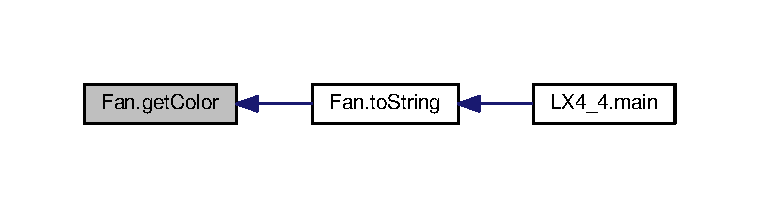
\includegraphics[width=350pt]{class_fan_a778ca7d0fdac62de6200efdd030c2d85_icgraph}
\end{center}
\end{figure}


\index{Fan@{Fan}!get\+On@{get\+On}}
\index{get\+On@{get\+On}!Fan@{Fan}}
\subsubsection[{\texorpdfstring{get\+On()}{getOn()}}]{\setlength{\rightskip}{0pt plus 5cm}boolean Fan.\+get\+On (
\begin{DoxyParamCaption}
{}
\end{DoxyParamCaption}
)\hspace{0.3cm}{\ttfamily [inline]}}\hypertarget{class_fan_ade7739493388a263603f8c8c931a79b7}{}\label{class_fan_ade7739493388a263603f8c8c931a79b7}


Definition at line 18 of file Fan.\+java.


\begin{DoxyCode}
18                            \{
19         \textcolor{keywordflow}{return} \hyperlink{class_fan_a59c1b7bdc39932e1283b4220255f4b80}{on};
20     \}
\end{DoxyCode}


Here is the caller graph for this function\+:
\nopagebreak
\begin{figure}[H]
\begin{center}
\leavevmode
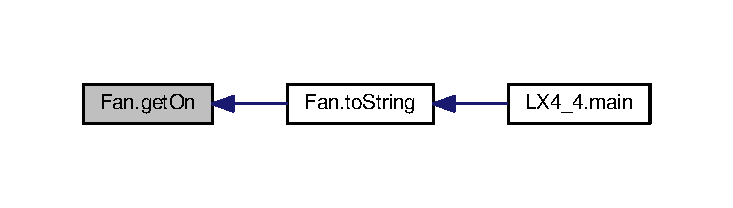
\includegraphics[width=350pt]{class_fan_ade7739493388a263603f8c8c931a79b7_icgraph}
\end{center}
\end{figure}


\index{Fan@{Fan}!get\+Radius@{get\+Radius}}
\index{get\+Radius@{get\+Radius}!Fan@{Fan}}
\subsubsection[{\texorpdfstring{get\+Radius()}{getRadius()}}]{\setlength{\rightskip}{0pt plus 5cm}double Fan.\+get\+Radius (
\begin{DoxyParamCaption}
{}
\end{DoxyParamCaption}
)\hspace{0.3cm}{\ttfamily [inline]}}\hypertarget{class_fan_a80c807d2d5415806393f6334188a42aa}{}\label{class_fan_a80c807d2d5415806393f6334188a42aa}


Definition at line 26 of file Fan.\+java.


\begin{DoxyCode}
26                               \{
27         \textcolor{keywordflow}{return} \hyperlink{class_fan_ae58060e831d9984859504bdc6f254c65}{radius};
28     \}
\end{DoxyCode}


Here is the caller graph for this function\+:
\nopagebreak
\begin{figure}[H]
\begin{center}
\leavevmode
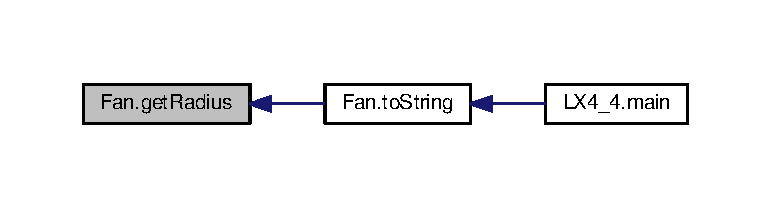
\includegraphics[width=350pt]{class_fan_a80c807d2d5415806393f6334188a42aa_icgraph}
\end{center}
\end{figure}


\index{Fan@{Fan}!get\+Speed@{get\+Speed}}
\index{get\+Speed@{get\+Speed}!Fan@{Fan}}
\subsubsection[{\texorpdfstring{get\+Speed()}{getSpeed()}}]{\setlength{\rightskip}{0pt plus 5cm}int Fan.\+get\+Speed (
\begin{DoxyParamCaption}
{}
\end{DoxyParamCaption}
)\hspace{0.3cm}{\ttfamily [inline]}}\hypertarget{class_fan_aa837e535d579b0ce52a18ee45165975b}{}\label{class_fan_aa837e535d579b0ce52a18ee45165975b}


Definition at line 10 of file Fan.\+java.


\begin{DoxyCode}
10                           \{
11         \textcolor{keywordflow}{return} \hyperlink{class_fan_af8aba46e1b2eb59022f1b89d07869d4b}{speed};
12     \}
\end{DoxyCode}


Here is the caller graph for this function\+:
\nopagebreak
\begin{figure}[H]
\begin{center}
\leavevmode
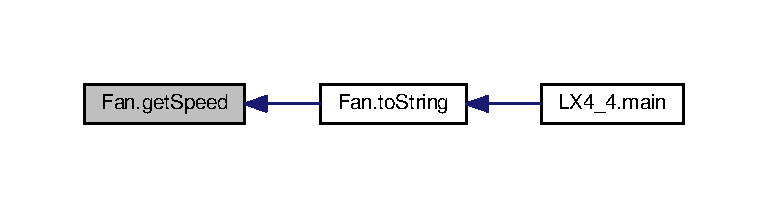
\includegraphics[width=350pt]{class_fan_aa837e535d579b0ce52a18ee45165975b_icgraph}
\end{center}
\end{figure}


\index{Fan@{Fan}!set\+Color@{set\+Color}}
\index{set\+Color@{set\+Color}!Fan@{Fan}}
\subsubsection[{\texorpdfstring{set\+Color(\+String a)}{setColor(String a)}}]{\setlength{\rightskip}{0pt plus 5cm}void Fan.\+set\+Color (
\begin{DoxyParamCaption}
\item[{String}]{a}
\end{DoxyParamCaption}
)\hspace{0.3cm}{\ttfamily [inline]}}\hypertarget{class_fan_afef0f6a39b56269a2592dcff067052d8}{}\label{class_fan_afef0f6a39b56269a2592dcff067052d8}


Definition at line 38 of file Fan.\+java.


\begin{DoxyCode}
38                                    \{
39         \hyperlink{class_fan_a2a06a2bf3c54f6afeee875c0daa801fa}{color} = a;
40     \}
\end{DoxyCode}


Here is the caller graph for this function\+:
\nopagebreak
\begin{figure}[H]
\begin{center}
\leavevmode
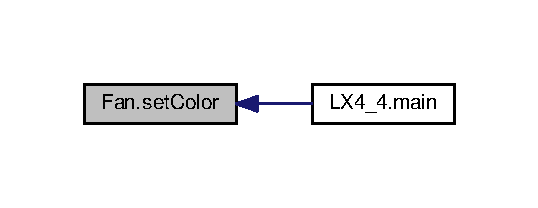
\includegraphics[width=258pt]{class_fan_afef0f6a39b56269a2592dcff067052d8_icgraph}
\end{center}
\end{figure}


\index{Fan@{Fan}!set\+On@{set\+On}}
\index{set\+On@{set\+On}!Fan@{Fan}}
\subsubsection[{\texorpdfstring{set\+On(boolean on1)}{setOn(boolean on1)}}]{\setlength{\rightskip}{0pt plus 5cm}void Fan.\+set\+On (
\begin{DoxyParamCaption}
\item[{boolean}]{on1}
\end{DoxyParamCaption}
)\hspace{0.3cm}{\ttfamily [inline]}}\hypertarget{class_fan_a4f7fd9e0ef71e219270d02ac36ad328b}{}\label{class_fan_a4f7fd9e0ef71e219270d02ac36ad328b}


Definition at line 22 of file Fan.\+java.


\begin{DoxyCode}
22                                    \{
23         \hyperlink{class_fan_a59c1b7bdc39932e1283b4220255f4b80}{on} = on1;
24     \}
\end{DoxyCode}


Here is the caller graph for this function\+:
\nopagebreak
\begin{figure}[H]
\begin{center}
\leavevmode
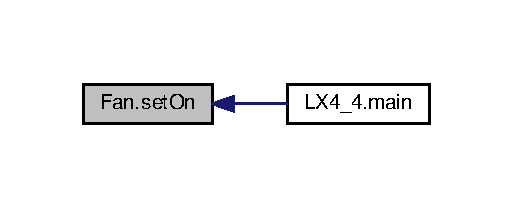
\includegraphics[width=246pt]{class_fan_a4f7fd9e0ef71e219270d02ac36ad328b_icgraph}
\end{center}
\end{figure}


\index{Fan@{Fan}!set\+Radius@{set\+Radius}}
\index{set\+Radius@{set\+Radius}!Fan@{Fan}}
\subsubsection[{\texorpdfstring{set\+Radius(double r)}{setRadius(double r)}}]{\setlength{\rightskip}{0pt plus 5cm}void Fan.\+set\+Radius (
\begin{DoxyParamCaption}
\item[{double}]{r}
\end{DoxyParamCaption}
)\hspace{0.3cm}{\ttfamily [inline]}}\hypertarget{class_fan_a13134b8be4efdd7403af98d763ce2199}{}\label{class_fan_a13134b8be4efdd7403af98d763ce2199}


Definition at line 30 of file Fan.\+java.


\begin{DoxyCode}
30                                     \{
31         \hyperlink{class_fan_ae58060e831d9984859504bdc6f254c65}{radius} = r;
32     \}
\end{DoxyCode}


Here is the caller graph for this function\+:
\nopagebreak
\begin{figure}[H]
\begin{center}
\leavevmode
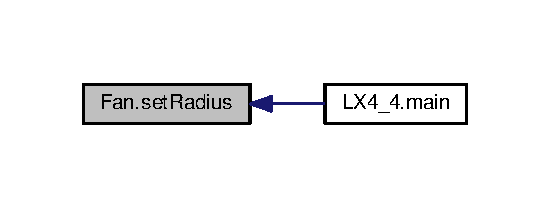
\includegraphics[width=264pt]{class_fan_a13134b8be4efdd7403af98d763ce2199_icgraph}
\end{center}
\end{figure}


\index{Fan@{Fan}!set\+Speed@{set\+Speed}}
\index{set\+Speed@{set\+Speed}!Fan@{Fan}}
\subsubsection[{\texorpdfstring{set\+Speed(int sp)}{setSpeed(int sp)}}]{\setlength{\rightskip}{0pt plus 5cm}void Fan.\+set\+Speed (
\begin{DoxyParamCaption}
\item[{int}]{sp}
\end{DoxyParamCaption}
)\hspace{0.3cm}{\ttfamily [inline]}}\hypertarget{class_fan_af95cee271f2412a52ac920f00b6ac90a}{}\label{class_fan_af95cee271f2412a52ac920f00b6ac90a}


Definition at line 14 of file Fan.\+java.


\begin{DoxyCode}
14                                  \{
15         \hyperlink{class_fan_af8aba46e1b2eb59022f1b89d07869d4b}{speed} = sp;
16     \}
\end{DoxyCode}


Here is the caller graph for this function\+:
\nopagebreak
\begin{figure}[H]
\begin{center}
\leavevmode
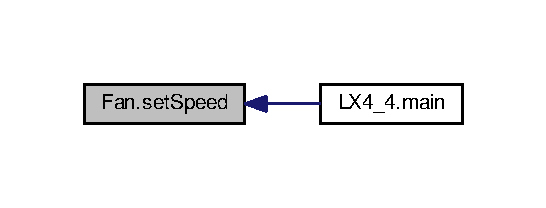
\includegraphics[width=262pt]{class_fan_af95cee271f2412a52ac920f00b6ac90a_icgraph}
\end{center}
\end{figure}


\index{Fan@{Fan}!to\+String@{to\+String}}
\index{to\+String@{to\+String}!Fan@{Fan}}
\subsubsection[{\texorpdfstring{to\+String()}{toString()}}]{\setlength{\rightskip}{0pt plus 5cm}String Fan.\+to\+String (
\begin{DoxyParamCaption}
{}
\end{DoxyParamCaption}
)\hspace{0.3cm}{\ttfamily [inline]}}\hypertarget{class_fan_a23b23cb45d15ed0e80d8a88c9300c5c6}{}\label{class_fan_a23b23cb45d15ed0e80d8a88c9300c5c6}


Definition at line 45 of file Fan.\+java.


\begin{DoxyCode}
45                              \{
46         \textcolor{keywordflow}{if} (this.\hyperlink{class_fan_ade7739493388a263603f8c8c931a79b7}{getOn}() == \textcolor{keyword}{true}) \{
47             \textcolor{keywordflow}{return} \textcolor{stringliteral}{"����ת�٣�"} + this.\hyperlink{class_fan_aa837e535d579b0ce52a18ee45165975b}{getSpeed}() + \textcolor{stringliteral}{"      ������ɫ��"} + this.
      \hyperlink{class_fan_a778ca7d0fdac62de6200efdd030c2d85}{getColor}()
48                     + \textcolor{stringliteral}{"  �뾶��"} + this.\hyperlink{class_fan_a80c807d2d5415806393f6334188a42aa}{getRadius}();
49         \} \textcolor{keywordflow}{else}
50             \textcolor{keywordflow}{return} \textcolor{stringliteral}{"fan is off"} + \textcolor{stringliteral}{"   ������ɫ��"} + this.\hyperlink{class_fan_a778ca7d0fdac62de6200efdd030c2d85}{getColor}() + \textcolor{stringliteral}{"     �뾶��"}
51                     + this.\hyperlink{class_fan_a80c807d2d5415806393f6334188a42aa}{getRadius}();
52     \}
\end{DoxyCode}


Here is the call graph for this function\+:
\nopagebreak
\begin{figure}[H]
\begin{center}
\leavevmode
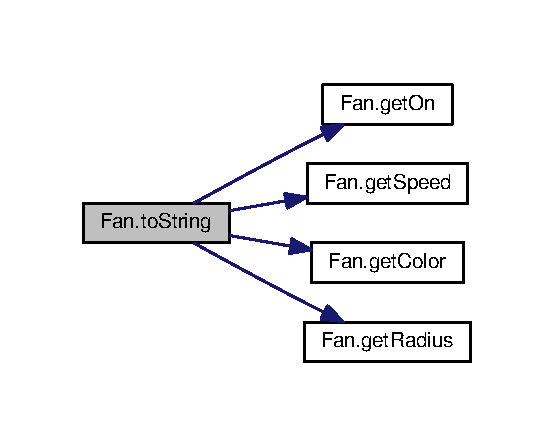
\includegraphics[width=266pt]{class_fan_a23b23cb45d15ed0e80d8a88c9300c5c6_cgraph}
\end{center}
\end{figure}




Here is the caller graph for this function\+:
\nopagebreak
\begin{figure}[H]
\begin{center}
\leavevmode
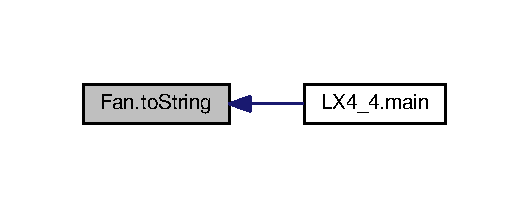
\includegraphics[width=254pt]{class_fan_a23b23cb45d15ed0e80d8a88c9300c5c6_icgraph}
\end{center}
\end{figure}




\subsection{Member Data Documentation}
\index{Fan@{Fan}!color@{color}}
\index{color@{color}!Fan@{Fan}}
\subsubsection[{\texorpdfstring{color}{color}}]{\setlength{\rightskip}{0pt plus 5cm}String Fan.\+color = \char`\"{}blue\char`\"{}\hspace{0.3cm}{\ttfamily [private]}}\hypertarget{class_fan_a2a06a2bf3c54f6afeee875c0daa801fa}{}\label{class_fan_a2a06a2bf3c54f6afeee875c0daa801fa}


Definition at line 8 of file Fan.\+java.

\index{Fan@{Fan}!fast@{fast}}
\index{fast@{fast}!Fan@{Fan}}
\subsubsection[{\texorpdfstring{fast}{fast}}]{\setlength{\rightskip}{0pt plus 5cm}final int Fan.\+fast = 3\hspace{0.3cm}{\ttfamily [static]}, {\ttfamily [package]}}\hypertarget{class_fan_a4220c2cd1983bacf972184a3cad21f91}{}\label{class_fan_a4220c2cd1983bacf972184a3cad21f91}


Definition at line 4 of file Fan.\+java.

\index{Fan@{Fan}!medium@{medium}}
\index{medium@{medium}!Fan@{Fan}}
\subsubsection[{\texorpdfstring{medium}{medium}}]{\setlength{\rightskip}{0pt plus 5cm}final int Fan.\+medium = 2\hspace{0.3cm}{\ttfamily [static]}, {\ttfamily [package]}}\hypertarget{class_fan_a9a1d7edabfa3efa358c2aa104e03cbe5}{}\label{class_fan_a9a1d7edabfa3efa358c2aa104e03cbe5}


Definition at line 3 of file Fan.\+java.

\index{Fan@{Fan}!on@{on}}
\index{on@{on}!Fan@{Fan}}
\subsubsection[{\texorpdfstring{on}{on}}]{\setlength{\rightskip}{0pt plus 5cm}boolean Fan.\+on = false\hspace{0.3cm}{\ttfamily [private]}}\hypertarget{class_fan_a59c1b7bdc39932e1283b4220255f4b80}{}\label{class_fan_a59c1b7bdc39932e1283b4220255f4b80}


Definition at line 6 of file Fan.\+java.

\index{Fan@{Fan}!radius@{radius}}
\index{radius@{radius}!Fan@{Fan}}
\subsubsection[{\texorpdfstring{radius}{radius}}]{\setlength{\rightskip}{0pt plus 5cm}double Fan.\+radius = 5\hspace{0.3cm}{\ttfamily [private]}}\hypertarget{class_fan_ae58060e831d9984859504bdc6f254c65}{}\label{class_fan_ae58060e831d9984859504bdc6f254c65}


Definition at line 7 of file Fan.\+java.

\index{Fan@{Fan}!slow@{slow}}
\index{slow@{slow}!Fan@{Fan}}
\subsubsection[{\texorpdfstring{slow}{slow}}]{\setlength{\rightskip}{0pt plus 5cm}final int Fan.\+slow = 1\hspace{0.3cm}{\ttfamily [static]}, {\ttfamily [package]}}\hypertarget{class_fan_a683c9a9821bd39be3cffdacf4132b79a}{}\label{class_fan_a683c9a9821bd39be3cffdacf4132b79a}


Definition at line 2 of file Fan.\+java.

\index{Fan@{Fan}!speed@{speed}}
\index{speed@{speed}!Fan@{Fan}}
\subsubsection[{\texorpdfstring{speed}{speed}}]{\setlength{\rightskip}{0pt plus 5cm}int Fan.\+speed = {\bf slow}\hspace{0.3cm}{\ttfamily [private]}}\hypertarget{class_fan_af8aba46e1b2eb59022f1b89d07869d4b}{}\label{class_fan_af8aba46e1b2eb59022f1b89d07869d4b}


Definition at line 5 of file Fan.\+java.



The documentation for this class was generated from the following file\+:\begin{DoxyCompactItemize}
\item 
source\+\_\+directory/fan/\hyperlink{_fan_8java}{Fan.\+java}\end{DoxyCompactItemize}

\hypertarget{class_l_x4__4}{}\section{L\+X4\+\_\+4 Class Reference}
\label{class_l_x4__4}\index{L\+X4\+\_\+4@{L\+X4\+\_\+4}}
\subsection*{Static Public Member Functions}
\begin{DoxyCompactItemize}
\item 
static void \hyperlink{class_l_x4__4_a6a062de65864f852990c51b8519919b0}{main} (String\mbox{[}$\,$\mbox{]} args)
\end{DoxyCompactItemize}


\subsection{Detailed Description}


Definition at line 1 of file L\+X4\+\_\+4.\+java.



\subsection{Member Function Documentation}
\index{L\+X4\+\_\+4@{L\+X4\+\_\+4}!main@{main}}
\index{main@{main}!L\+X4\+\_\+4@{L\+X4\+\_\+4}}
\subsubsection[{\texorpdfstring{main(\+String[] args)}{main(String[] args)}}]{\setlength{\rightskip}{0pt plus 5cm}static void L\+X4\+\_\+4.\+main (
\begin{DoxyParamCaption}
\item[{String\mbox{[}$\,$\mbox{]}}]{args}
\end{DoxyParamCaption}
)\hspace{0.3cm}{\ttfamily [inline]}, {\ttfamily [static]}}\hypertarget{class_l_x4__4_a6a062de65864f852990c51b8519919b0}{}\label{class_l_x4__4_a6a062de65864f852990c51b8519919b0}


Definition at line 2 of file L\+X4\+\_\+4.\+java.


\begin{DoxyCode}
2                                            \{
3         \hyperlink{class_fan}{Fan} fan1 = \textcolor{keyword}{new} \hyperlink{class_fan}{Fan}();
4         fan1.\hyperlink{class_fan_af95cee271f2412a52ac920f00b6ac90a}{setSpeed}(3);
5         fan1.\hyperlink{class_fan_a13134b8be4efdd7403af98d763ce2199}{setRadius}(10);
6         fan1.\hyperlink{class_fan_afef0f6a39b56269a2592dcff067052d8}{setColor}(\textcolor{stringliteral}{"yellow"});
7         fan1.\hyperlink{class_fan_a4f7fd9e0ef71e219270d02ac36ad328b}{setOn}(\textcolor{keyword}{true});
8         \hyperlink{class_fan}{Fan} fan2 = \textcolor{keyword}{new} \hyperlink{class_fan}{Fan}();
9         fan2.\hyperlink{class_fan_af95cee271f2412a52ac920f00b6ac90a}{setSpeed}(2);
10         fan2.\hyperlink{class_fan_a13134b8be4efdd7403af98d763ce2199}{setRadius}(5);
11         fan2.\hyperlink{class_fan_afef0f6a39b56269a2592dcff067052d8}{setColor}(\textcolor{stringliteral}{"blue"});
12         fan2.\hyperlink{class_fan_a4f7fd9e0ef71e219270d02ac36ad328b}{setOn}(\textcolor{keyword}{false});
13         System.out.println(fan1.\hyperlink{class_fan_a23b23cb45d15ed0e80d8a88c9300c5c6}{toString}());
14         System.out.println(fan2.\hyperlink{class_fan_a23b23cb45d15ed0e80d8a88c9300c5c6}{toString}());
15     \}
\end{DoxyCode}


Here is the call graph for this function\+:
\nopagebreak
\begin{figure}[H]
\begin{center}
\leavevmode
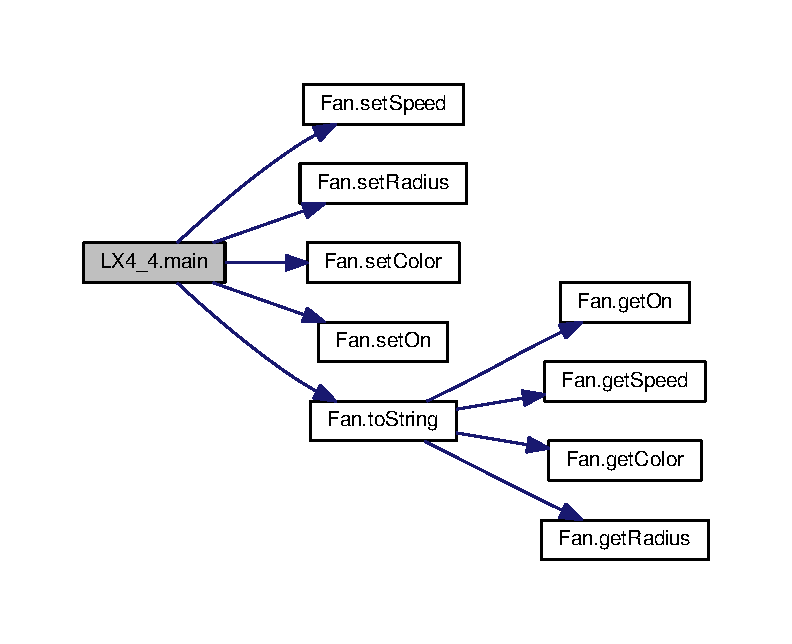
\includegraphics[width=350pt]{class_l_x4__4_a6a062de65864f852990c51b8519919b0_cgraph}
\end{center}
\end{figure}




The documentation for this class was generated from the following file\+:\begin{DoxyCompactItemize}
\item 
source\+\_\+directory/fan/\hyperlink{_l_x4__4_8java}{L\+X4\+\_\+4.\+java}\end{DoxyCompactItemize}

\chapter{File Documentation}
\hypertarget{_fan_8java}{}\section{source\+\_\+directory/fan/\+Fan.java File Reference}
\label{_fan_8java}\index{source\+\_\+directory/fan/\+Fan.\+java@{source\+\_\+directory/fan/\+Fan.\+java}}
\subsection*{Classes}
\begin{DoxyCompactItemize}
\item 
class \hyperlink{class_fan}{Fan}
\end{DoxyCompactItemize}

\hypertarget{_l_x4__4_8java}{}\section{source\+\_\+directory/fan/\+L\+X4\+\_\+4.java File Reference}
\label{_l_x4__4_8java}\index{source\+\_\+directory/fan/\+L\+X4\+\_\+4.\+java@{source\+\_\+directory/fan/\+L\+X4\+\_\+4.\+java}}
\subsection*{Classes}
\begin{DoxyCompactItemize}
\item 
class \hyperlink{class_l_x4__4}{L\+X4\+\_\+4}
\end{DoxyCompactItemize}

%--- End generated contents ---

% Index
\backmatter
\newpage
\phantomsection
\clearemptydoublepage
\addcontentsline{toc}{chapter}{Index}
\printindex

\end{document}
